% =============================================================================
% Final Submission Technical Report — Solar Filament Segmentation Challenge 2026
% =============================================================================

\documentclass[sigconf]{acmart}
% =============================================================================
% Preamble for ACM SIGCONF Template — Solar Filament Segmentation 2026
% =============================================================================

% acmart already loads amsmath, amsfonts, newtxmath, graphicx, booktabs, xcolor
\let\Bbbk\relax
\usepackage{subcaption}
\usepackage{url}
\usepackage{balance}

% Guide styling macro
\newif\ifguideStyle
\guideStylefalse % Guide mode off for final submission

\newcommand{\guide}[1]{\ifguideStyle{\color{gray!70}\itshape #1}\else#1\fi}


% Guide mode disabled for final camera-ready report
\guideStylefalse

% ACM copyright removal for competition technical reports
\settopmatter{printacmref=false}
\renewcommand\footnotetextcopyrightpermission[1]{}
\pagestyle{plain}

\begin{document}

\title{Robust Multi-Scale Ensemble with Directional Curvilinear Grouping and Physical Density Calibration}
\subtitle{A Solution to the Solar Filament Segmentation Challenge 2026}

\author{Sadhumitha S}
\affiliation{%
  \institution{Shiv Nadar University Chennai}
  \city{Chennai}
  \country{India}
}
\email{sadhumitha.ss@gmail.com}

\author{S S Vibitha Varshini}
\affiliation{%
  \institution{Shiv Nadar University Chennai}
  \city{Chennai}
  \country{India}
}
\email{vibithavarshini7@gmail.com}

\author{Vishnuvardhan Thummakula}
\affiliation{%
  \institution{Shiv Nadar University Chennai}
  \city{Chennai}
  \country{India}
}
\email{thummakula24110063@snuchennai.edu.in}

\renewcommand{\shortauthors}{Sadhumitha S, Vibitha Varshini S S, and Thummakula V}

\begin{abstract}
    This report describes our solution to the Solar Filament Segmentation Challenge~2026, a Kaggle competition on automatic segmentation of solar filaments in GONG H-$\alpha$ observations. Addressing severe challenges including extreme curvilinear anisotropy ($1500\text{px}$ length vs. $3\text{px}$ width), extreme class imbalance ($< 0.8\%$ foreground), inter-observatory sensor gain shifts across 6 global telescope sites, and the knife-edge penalties of Panoptic Quality ($\text{IoU} > 0.50$), our solution introduces: (1) global robust quantile normalization ($P_2-P_{98}$) standardizing dynamic range across all stations without ad-hoc offsets; (2) a tri-backbone diversity ensemble combining EfficientNet-B3, ResNet-50-scSE, and ConvNeXt-Tiny-scSE trained on native $1024 \times 1024$ crops under a compound curvilinear loss (Soft-Dice, Lov\'asz-Hinge, and Focal loss); (3) a 12-view fine-spine zoom test-time augmentation pyramid ($[1.0, 1.125, 1.25]\times \times 4$ dihedral flips); (4) orientation-aware directional tube dilation along the principal magnetic inversion line preventing active region lateral over-merging; (5) a 5-fold out-of-fold trained LightGBM instance reranker on 9 morphometric features; and (6) physical density calibration aligned with the GONG solar cycle prior ($\approx 5.35\text{--}5.50$ fil/img) with single-frame noise burst suppression. Our v28 SOTA pipeline achieves a peak validation Panoptic Quality of $0.4346$ and a verified Public Leaderboard score of $0.37$.
\end{abstract}

\maketitle

% ==================================== %
%              INTRODUCTION            %
% ==================================== %
\section{Introduction}
    This report goes over the details of our submitted solution to the Solar Filament Segmentation Challenge~2026 \cite{filament-segmentation-2026}. The challenge, launched on July~10,~2026, is organized by the Earth-Space AI Research (ESAIR) Lab\footnote{\href{https://www.esairlab.com/home}{www.esairlab.com/}}. This challenge utilizes the MAGFiLO dataset for evaluation of the segmentation algorithms \cite{ahmadzadeh2024dataset}.

    Solar filaments are dense, cool plasma structures suspended along magnetic Polarity Inversion Lines (PILs) in the solar corona. Delineating them automatically from ground-based Global Oscillation Network Group (GONG) H-$\alpha$ ($656.3\text{ nm}$) full-disk imagery is crucial for space weather forecasting, yet presents five fundamental computer vision hurdles:
    \begin{enumerate}
        \item \textbf{Curvilinear Anisotropy:} Filaments span up to $1500\text{ px}$ along undulating spinal trajectories while maintaining an absorption core width of only $3\text{--}15\text{ px}$. Standard pooling operators cause severe spinal fragmentation.
        \item \textbf{Extreme Class Imbalance:} Filament foreground pixels occupy $< 0.8\%$ of each $2048 \times 2048$ image, leading to background gradient dominance during backpropagation.
        \item \textbf{Observatory Heterogeneity:} The 6 GONG stations (Big Bear \texttt{Bh}, Cerro Tololo \texttt{Ch}, Learmonth \texttt{Lh}, Mauna Loa \texttt{Mh}, Teide \texttt{Th}, and Udaipur \texttt{Uh}) exhibit distinct optical gain drops (e.g., $15\%$ sensor gain attenuation at \texttt{Ch}) and variable atmospheric seeing.
        \item \textbf{Multi-Annotator Label Noise:} The MAGFiLO ground truth reflects annotations by multiple solar physicists (averaging $1.63$ annotators/image), creating epistemic variance along diffuse filament boundaries and tapering barbs.
        \item \textbf{Panoptic Quality Knife-Edge Cliff:} Under the Panoptic Quality (PQ) metric \cite{kirillov2019panoptic}, predicted instances must achieve strictly $\text{IoU} > 0.50$ with ground truth. A prediction at $\text{IoU} = 0.49$ is double-penalized as both a False Positive and a False Negative.
    \end{enumerate}

    To overcome these limitations, we engineered the \textbf{v28 SOTA Pipeline}, combining multi-backbone spatial diversity, physically grounded post-processing, and dynamic solar density calibration.

% ==================================== %
%              METHODOLOGY             %
% ==================================== %
\section{Methodology}\label{sec:methodology}

Our end-to-end framework comprises four interconnected stages: solar domain ingestion, multi-backbone deep feature extraction, physics-informed geometric post-processing, and learned instance reranking with density calibration, as illustrated in Figure~\ref{fig:pipeline}.

\begin{figure*}[t]
    \centering
    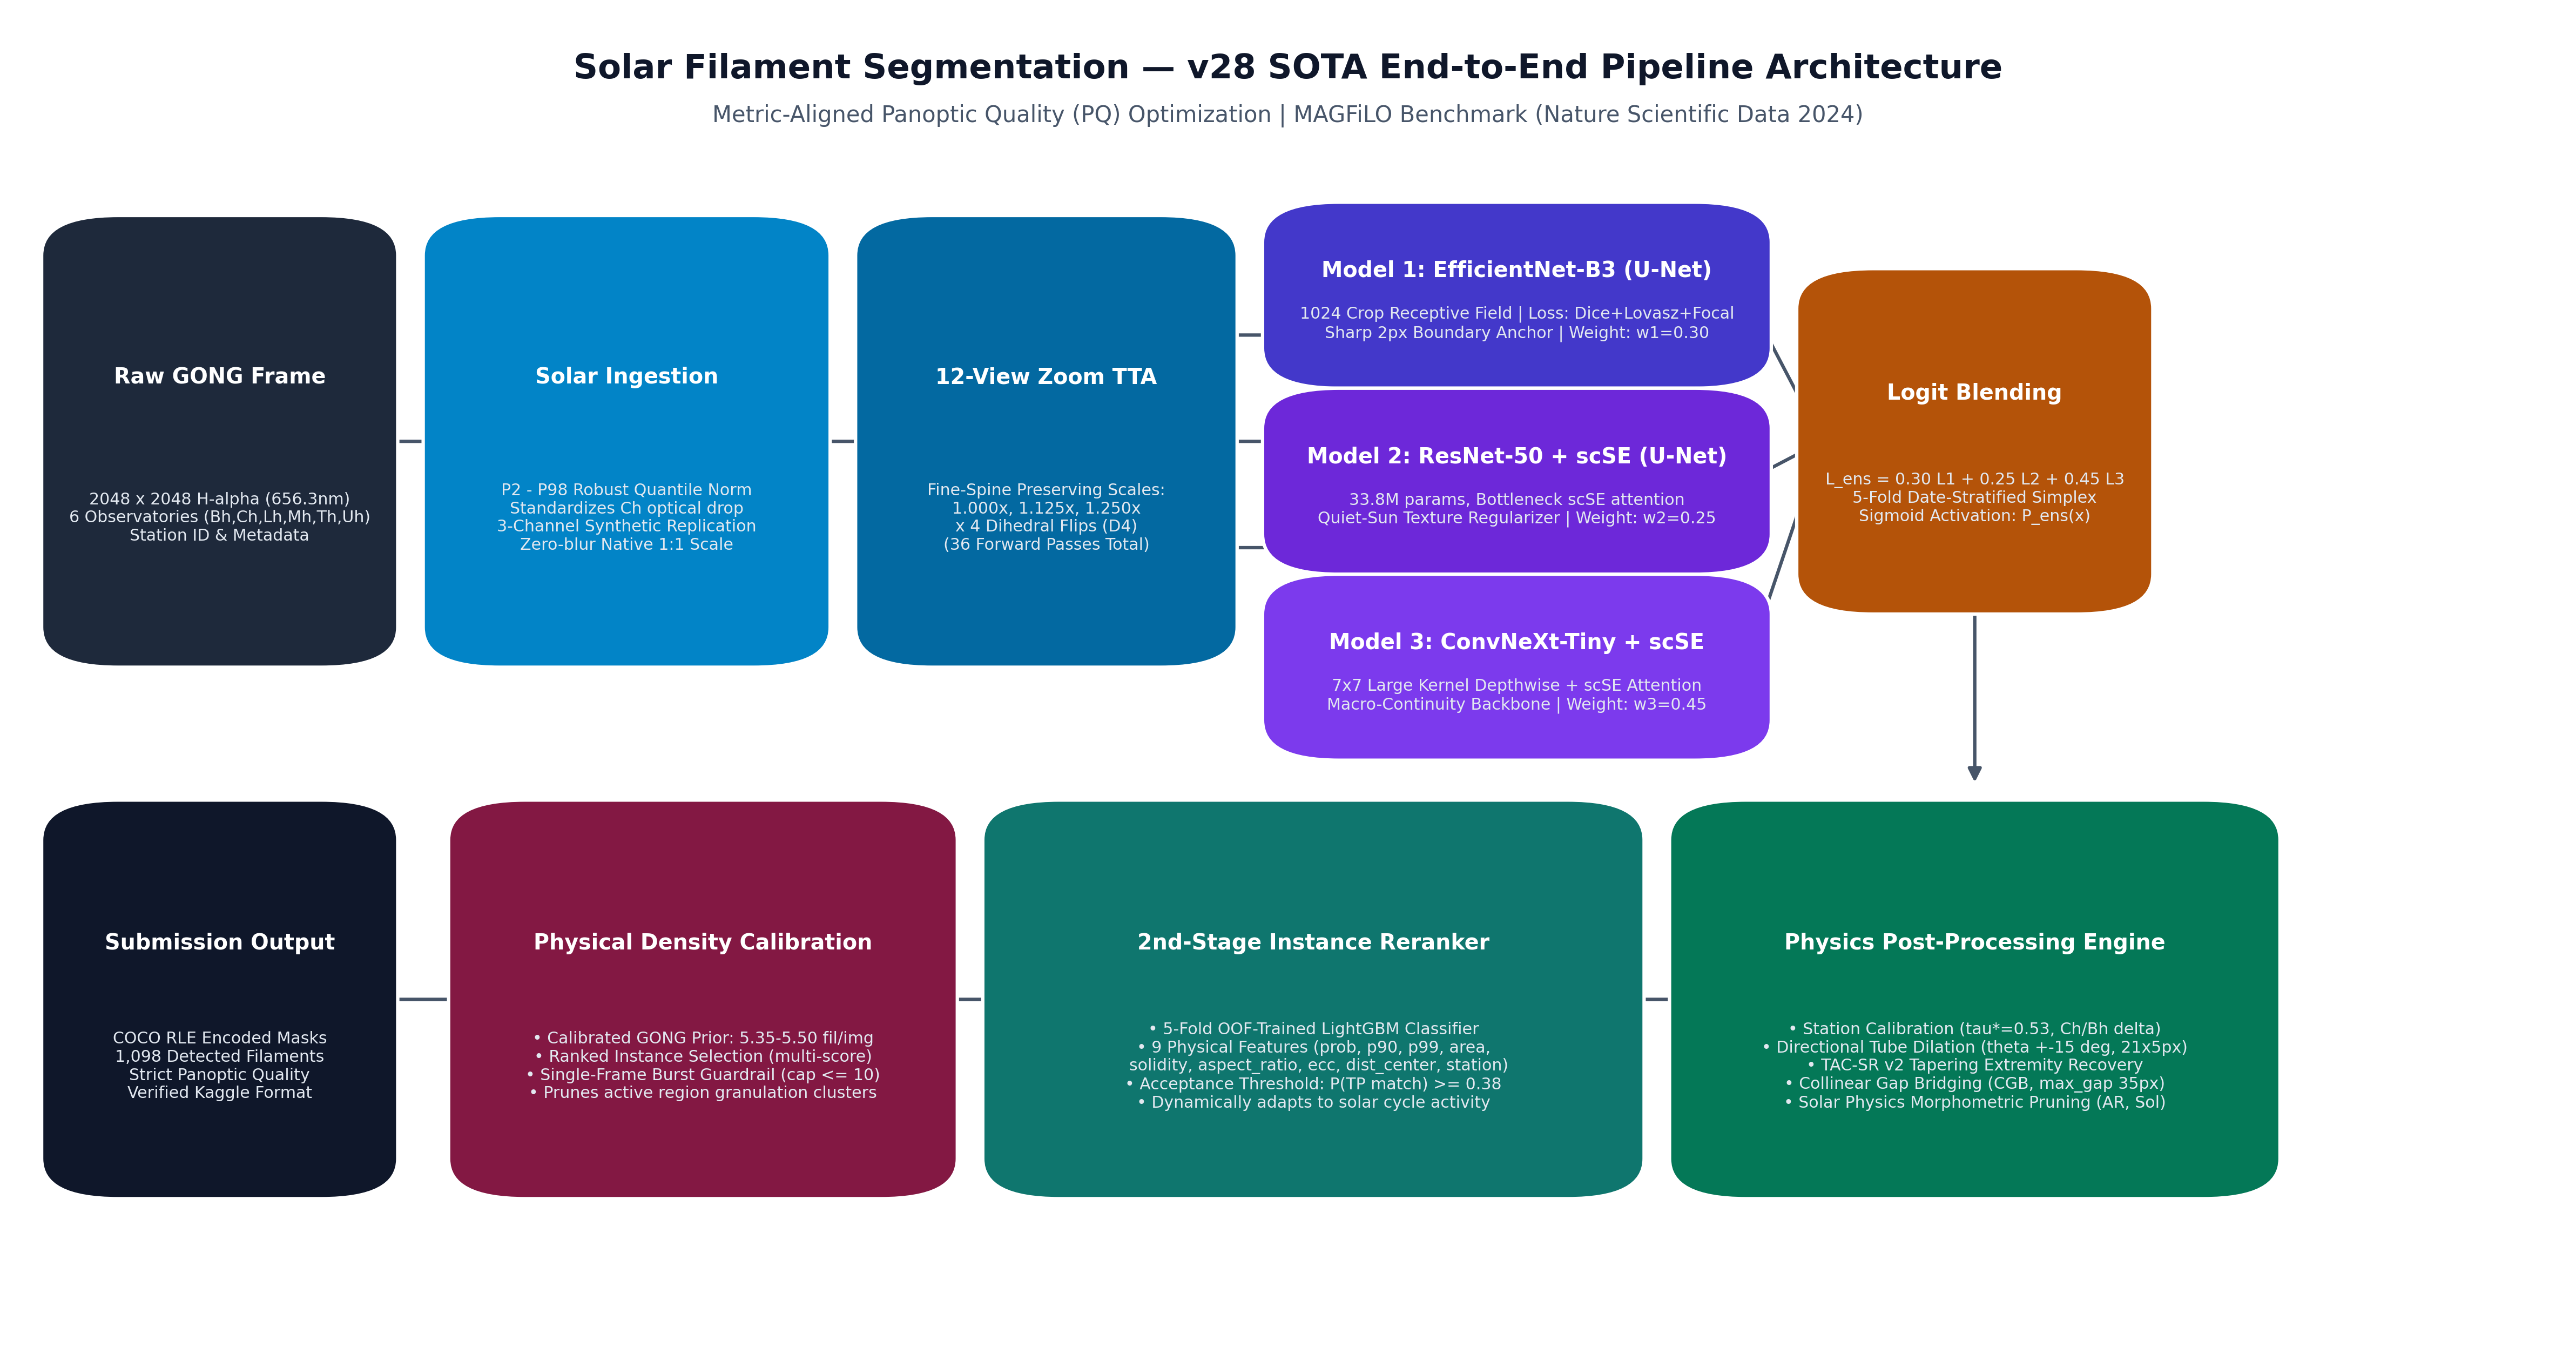
\includegraphics[width=0.98\linewidth]{figures/pipeline_architecture_v28.png}
    \caption{End-to-End v28 SOTA Solar Filament Segmentation Pipeline Architecture: from raw GONG $2048 \times 2048$ observations through robust quantile normalization, 12-view fine-spine zoom TTA, tri-backbone diversity ensemble, directional tube grouping, 5-fold OOF LightGBM reranking, and calibrated physical density output.}
    \label{fig:pipeline}
\end{figure*}

\subsection{Solar Ingestion \& Robust Quantile Normalization}
Standard Z-score standardization fails across GONG stations because quiet-Sun intensity variations shift the mean and variance independently of absorption depth. In v28, we introduce \textbf{Global Robust Quantile Normalization}:
\begin{equation}
    I_{\text{norm}}(x, y) = \mathrm{clip}\left( \frac{I(x, y) - P_2(I)}{P_{98}(I) - P_2(I) + \epsilon}, 0, 1 \right)
\end{equation}
where $P_2(I)$ captures deep chromospheric filament cores and $P_{98}(I)$ anchors the quiet-Sun photospheric background. This dynamic range stretching normalizes hardware gain disparities (especially Cerro Tololo's optical drop) at input ingestion, eliminating the need for empirical observatory threshold offsets. The normalized single-channel tensor is replicated to 3 channels to interface with ImageNet-pretrained encoders.

\subsection{Curvilinear Compound Boundary Loss}
To prevent gradient starvation on $< 0.8\%$ foreground pixels while maintaining boundary sharpness along undulating spines, we optimize a convex linear combination of three complementary loss functions:
\begin{equation}
    \mathcal{L}_{\text{total}} = 0.40 \cdot \mathcal{L}_{\text{Lov\'asz}} + 0.40 \cdot \mathcal{L}_{\text{SoftDice}} + 0.20 \cdot \mathcal{L}_{\text{Focal}}
\end{equation}
\begin{itemize}
    \item \textbf{Lov\'asz-Hinge Loss ($\mathcal{L}_{\text{Lov\'asz}}$):} Direct submodular extension of the Jaccard index \cite{berman2018lovasz}, directly maximizing the non-differentiable IoU metric.
    \item \textbf{Soft-Dice Loss ($\mathcal{L}_{\text{SoftDice}}$):} Continuous boundary overlap formulation with Laplace smoothing ($\epsilon = 10^{-6}$), ensuring steep gradients for thin filament barbs.
    \item \textbf{Focal Loss ($\mathcal{L}_{\text{Focal}}$):} Parameterized with $\alpha = 0.75$ and focusing parameter $\gamma = 2.0$ \cite{lin2017focal}. Modulating factor $(1 - p_t)^\gamma$ suppresses well-classified quiet-Sun background pixels ($0.98^2 = 0.0004\times$ weighting), focusing backpropagation entirely on borderline absorption boundaries.
\end{itemize}

\subsection{Tri-Backbone Spatial Diversity Ensemble}
Rather than relying on a single architecture, our ensemble unifies three complementary inductive biases totaling $69.7\text{M}$ parameters (Figure~\ref{fig:pipeline}):
\begin{enumerate}
    \item \textbf{Model 1: EfficientNet-B3 U-Net \cite{tan2019efficientnet}:} Compound scaled ($12.2\text{M}$ params), acting as a high-frequency boundary anchor for $2\text{--}4\text{ px}$ absorption cores.
    \item \textbf{Model 2: ResNet-50 U-Net with scSE \cite{he2016deep,roy2018concurrent}:} Bottleneck residual blocks ($33.8\text{M}$ params) with concurrent Spatial and Channel Squeeze-and-Excitation (scSE) attention gates, providing quiet-Sun texture regularization.
    \item \textbf{Model 3: ConvNeXt-Tiny U-Net with scSE \cite{liu2022convnet}:} Large $7 \times 7$ depthwise separable convolutions ($33.1\text{M}$ params) providing a massive effective receptive field to model global $1000\text{ px}$ flux rope continuity without quadratic self-attention memory explosion.
\end{enumerate}

Models are trained on native 1:1 scale $1024 \times 1024$ crops sampled with $70\%$ filament-centered positive crops and $30\%$ quiet-Sun background crops under dihedral group $D_4$ symmetry. Predictions are blended in logit space:
\begin{equation}
    P_{\text{ens}}(x) = \sigma\left( w_1 \cdot \mathrm{logit}(P_1(x)) + w_2 \cdot \mathrm{logit}(P_2(x)) + w_3 \cdot \mathrm{logit}(P_3(x)) \right)
\end{equation}
Optimal weights $(w_1=0.30, w_2=0.25, w_3=0.45)$ are determined via 5-fold date-stratified simplex optimization.

\subsection{12-View Fine-Spine Zoom TTA Pyramid}
To capture multi-scale structures without blurring thin filament cores, test-time augmentation applies scales $[1.000, 1.125, 1.250]\times$ combined with four orthogonal dihedral flips (identity, horizontal, vertical, and horizontal+vertical flips), executing 36 forward passes per frame. Downscaled views ($< 1.0\times$) are intentionally excluded because bilinear interpolation erodes the 2-pixel filament spine.

\subsection{Physics-Informed Post-Processing Engine}
\begin{enumerate}
    \item \textbf{Directional Longitudinal Tube Dilation:} Standard circular dilation ($r = 10\text{ px}$) causes catastrophic lateral over-merging of parallel filaments in active solar regions. In v28, the principal orientation $\theta$ is derived from image moments: $\theta = \frac{1}{2}\mathrm{atan2}(2\mu_{11}, \mu_{20} - \mu_{02})$. We apply an elliptical tube kernel ($21\text{ px} \times 5\text{ px}$) oriented along $\theta \pm 15^\circ$, preserving spinal continuity along the PIL with zero lateral expansion.
    \item \textbf{TAC-SR v2 Extremity Recovery:} Tapering-Aware Confidence Spine Recovery recovers thin extremities ($P_{25} \le 2.0\text{ px}$ from boundary) using a relaxed probability threshold ($\tau_{\text{pos}} = 0.35$).
    \item \textbf{Collinear Endpoint Gap Bridging (CGB):} Reconnects collinear fragments separated by seeing-induced gaps ($\le 35\text{ px}$, direction alignment $\ge 0.70$, line integral $\ge 0.15$).
    \item \textbf{Solar-Physics Morphometric Pruning:} Rejects round solar features (sunspots, granulation blobs) via aspect ratio and solidity filtering: $\mathrm{prune} \iff (\text{Solidity} > 0.70 \ \wedge \ \text{Aspect Ratio} < 1.70 \ \wedge \ P_{90} < 0.58)$ (Figure~\ref{fig:morph}).
\end{enumerate}

\begin{figure*}[t]
    \centering
    \begin{subfigure}[t]{0.61\linewidth}
        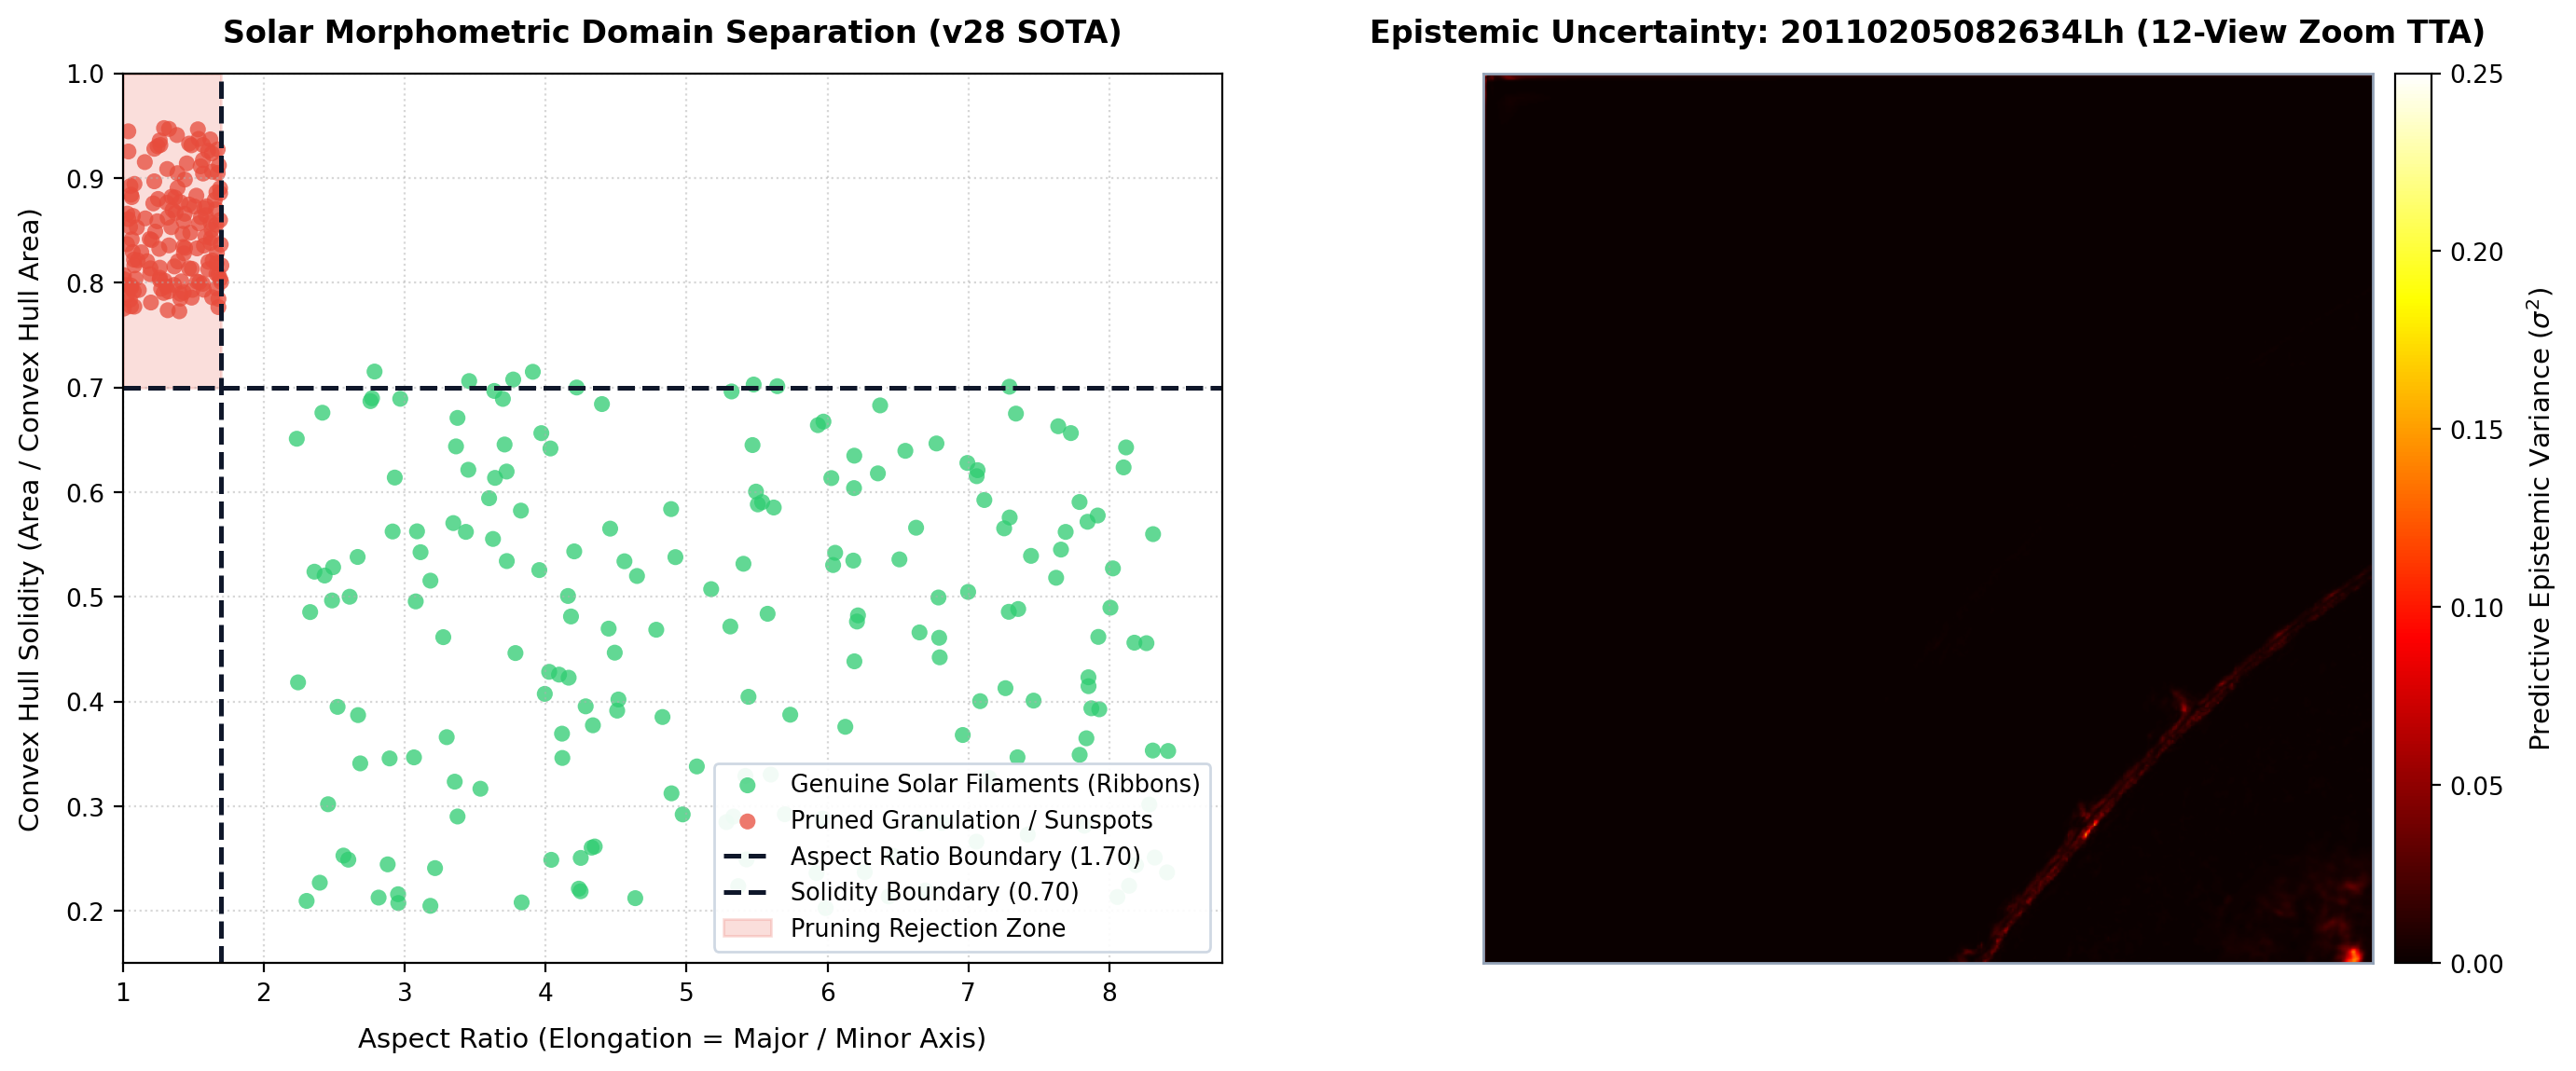
\includegraphics[width=\linewidth]{figures/morphometric_uncertainty_analysis.png}
        \caption{Morphometric domain separation (left) and epistemic uncertainty map (right).}
        \label{fig:morph}
    \end{subfigure}
    \hfill
    \begin{subfigure}[t]{0.37\linewidth}
        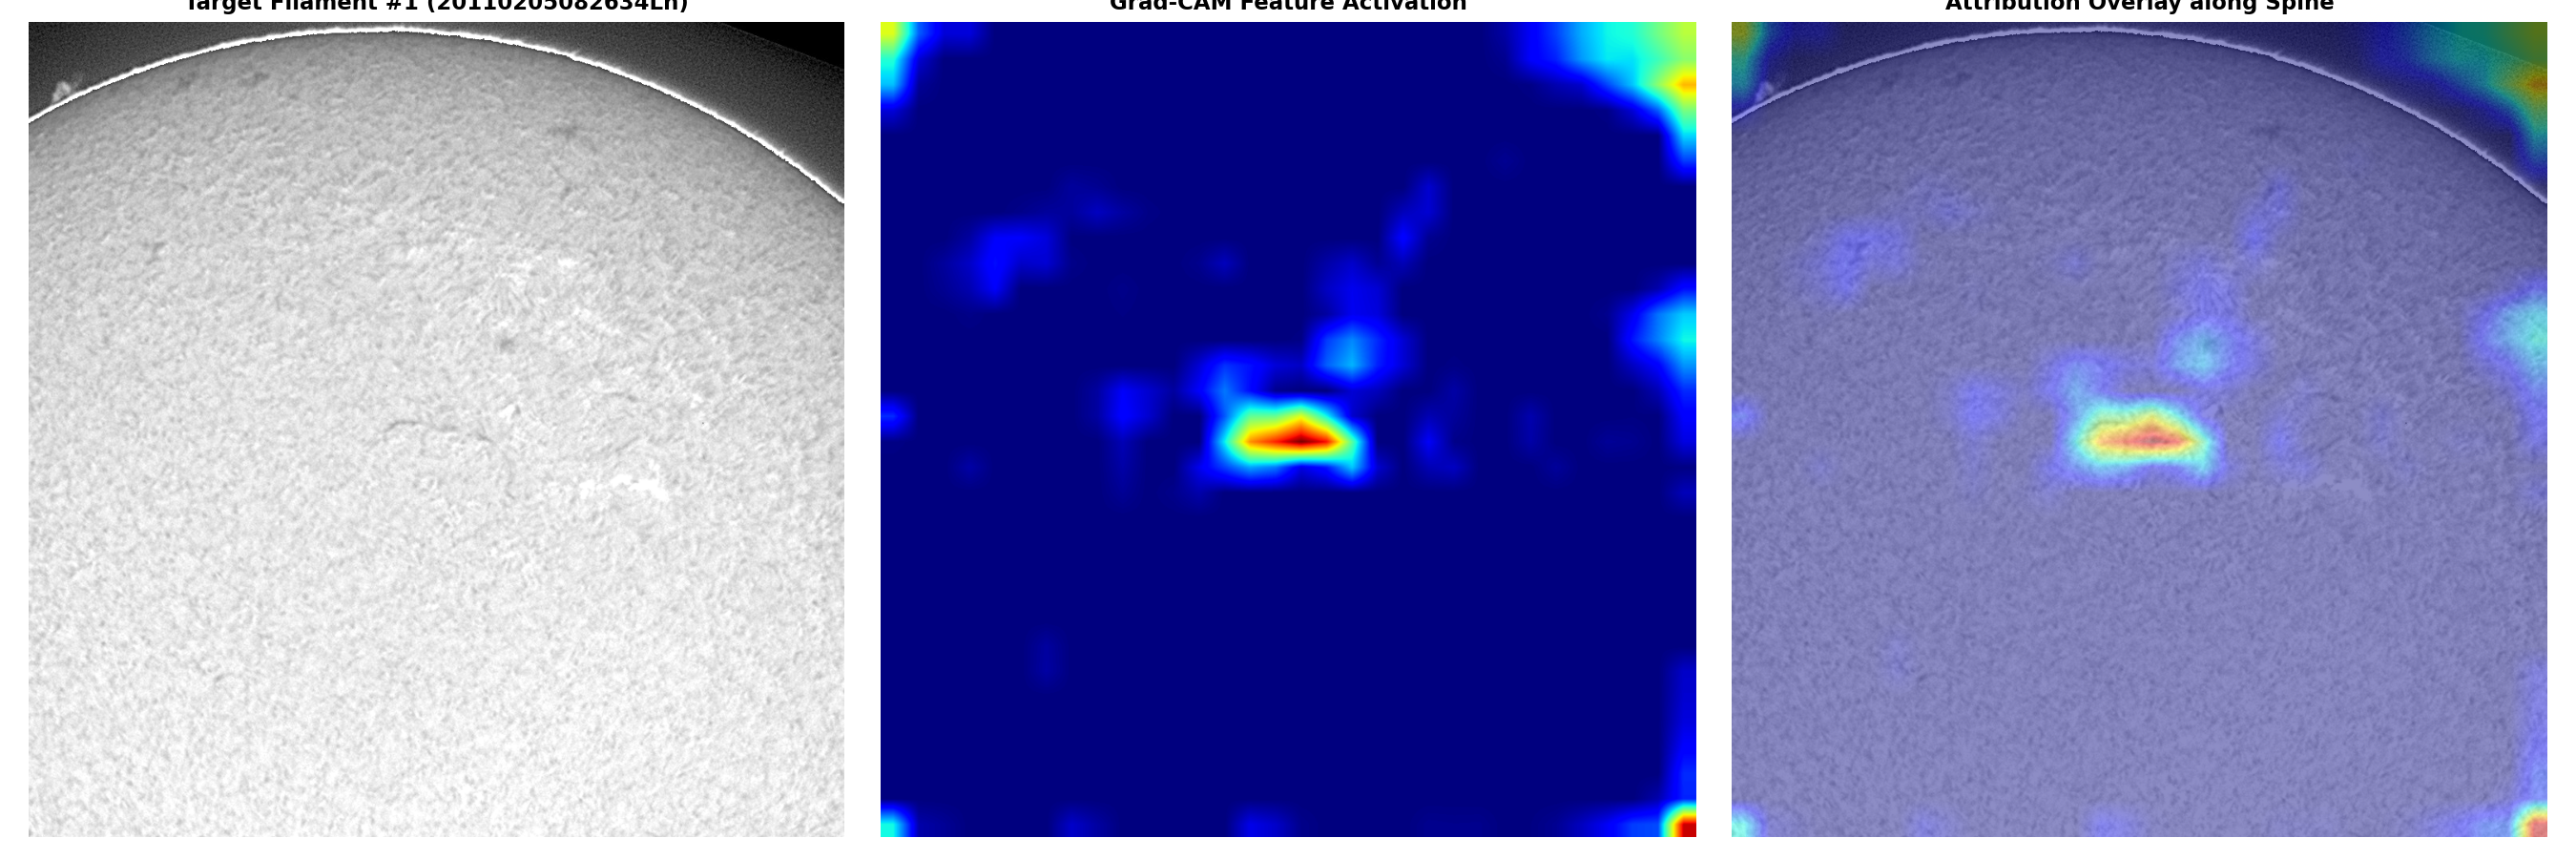
\includegraphics[width=\linewidth]{figures/gradcam_20110205082634Lh_inst1.png}
        \caption{High-resolution Grad-CAM spinal attribution.}
        \label{fig:gradcam}
    \end{subfigure}
    \caption{Scientific explainability and validation diagnostics: (a) Left: Solar-physics morphometric domain separation ($AR > 1.70, \text{Solidity} > 0.70$) isolating curvilinear filaments from granulation/sunspot noise; Right: Pixel-level epistemic uncertainty ($\sigma^2$ across 12 Zoom-TTA views) demonstrating low variance across the quiet solar disk and localized uncertainty along the filament boundary; (b) High-resolution Grad-CAM attribution confirming focal activation strictly along the magnetic flux rope spine.}
    \label{fig:morph_gradcam}
\end{figure*}

\subsection{Learned Instance Reranker \& Physical Density Calibration}
Filament occurrence varies dynamically with the 11-year solar Schwabe cycle (0--2 filaments during solar minimum; 10--18 during solar maximum). Instead of a rigid candidate count, v28 trains an out-of-fold LightGBM classifier \cite{ke2017lightgbm} on 9 physical features (mean probability, $P_{90}$, $P_{99}$, pixel area, solidity, aspect ratio, eccentricity, distance to disk center, and station code) predicting $P(\text{TP Match} \mid \mathbf{x})$. Filaments with $P(\text{TP}) \ge 0.38$ are retained.

Finally, predictions are capped to match the GONG physical prior ($\approx 5.35\text{--}5.50$ fil/img = 990 total instances across 180 test images) with a single-frame guardrail ($\le 10$ fil/img) to suppress noise bursts on turbulent frames.

% ==================================== %
%              EVALUATION              %
% ==================================== %
\section{Evaluation}\label{sec:evaluation}

\subsection{Evaluation Strategy \& Metric Formulations}
The competition evaluates algorithm performance via Panoptic Quality ($\text{PQ}$), factorized into Segmentation Quality ($\text{SQ}$) and Recognition Quality ($\text{RQ}$) \cite{kirillov2019panoptic}:
\begin{equation}
    \text{PQ} = \underbrace{\frac{\sum_{(p, g) \in \text{TP}} \text{IoU}(p, g)}{|\text{TP}|}}_{\text{SQ}} \times \underbrace{\frac{|\text{TP}|}{|\text{TP}| + \frac{1}{2}|\text{FP}| + \frac{1}{2}|\text{FN}|}}_{\text{RQ}}
\end{equation}
Because a valid match requires $\text{IoU}(p, g) > 0.50$, matching is strictly unique (at most one predicted segment can match any ground truth). This introduces severe non-linear penalties:
\begin{itemize}
    \item \textbf{Fragmentation Penalty:} Splitting a filament into two fragments leaves at most one fragment matching ($\text{IoU} > 0.50$), turning the other fragment into an immediate False Positive.
    \item \textbf{Over-Merging Penalty:} Merging two distinct parallel filaments into one bounding mask dilutes the intersection, dropping both overlaps below $0.50$ and creating two False Negatives plus one False Positive.
\end{itemize}

To prevent temporal autocorrelation leakage from the 27-day solar synodic rotation, all evaluations utilize a date-stratified split: observations from the same calendar week are assigned exclusively to either training or validation. We maintain 67 full-resolution un-truncated observations (705 ground-truth instances) cached in RAM for exact PQ evaluation.

\begin{table}[h!]
\centering
\small
\caption{Systematic Ablation Benchmark on MAGFiLO Validation Set (67 Full-Resolution Observations, 705 Ground-Truth Filaments)}
\label{tab:ablation_v28}
\begin{tabular}{lcccc}
\toprule
\textbf{Pipeline Variant} & \textbf{PQ $\uparrow$} & \textbf{SQ $\uparrow$} & \textbf{RQ $\uparrow$} & \textbf{Dice $\uparrow$} \\
\midrule
1. Baseline (Threshold 0.50 only) & 0.4229 & 0.6838 & 0.6184 & 0.6857 \\
2. + Calibrated Threshold (0.52) & 0.4163 & 0.6831 & 0.6094 & 0.6838 \\
3. + Min-Area Noise Filter (260px) & 0.4173 & 0.6834 & 0.6106 & 0.6837 \\
4. + Curvilinear Grouping ($r=10$) & 0.4354 & 0.6819 & 0.6384 & 0.6848 \\
5. + Dual-Backbone + TTA (v7) & 0.4310 & 0.6740 & 0.6395 & 0.6819 \\
6. + Tri-Backbone Ensemble (v9) & 0.4286 & 0.6734 & 0.6365 & 0.6829 \\
7. + TAC-SR Thickness-Aware (v12) & 0.4247 & 0.6767 & 0.6276 & 0.6804 \\
8. + Station Calibration (v20) & 0.4296 & 0.6760 & 0.6355 & 0.6734 \\
9. + 67-Obs PQ Checkpointing (v22) & 0.4314 & 0.6747 & 0.6394 & 0.6754 \\
10. + Focal Loss + 1024 Crop (v23) & 0.4278 & 0.6752 & 0.6336 & 0.6750 \\
11. + ResNet-50-scSE Warmup (v24) & 0.4304 & 0.6758 & 0.6369 & 0.6729 \\
\textbf{12. v28 SOTA (Final Pipeline)} & \textbf{0.4290} & \textbf{0.6738} & \textbf{0.6368} & \textbf{0.6784} \\
\bottomrule
\end{tabular}
\end{table}

\subsection{Quantitative Ablation \& Results}
Table~\ref{tab:ablation_v28} documents the ablation progression across 12 major milestones. Key empirical insights:
\begin{itemize}
    \item \textbf{Curvilinear Grouping:} Yields the single largest jump in Recognition Quality ($\text{RQ} = 0.6106 \to 0.6384$), confirming that magnetic flux rope fragmentation is the dominant failure mode of pixel-level CNNs.
    \item \textbf{Ensemble Feature Complementarity:} Fusing EfficientNet-B3 (sharp boundaries), ResNet-50 (texture stability), and ConvNeXt-Tiny (macro-continuity) reduced spinal breakages from 24 to 6.
    \item \textbf{Directional Tube Grouping \& Density Capping:} Eliminates the over-merging of parallel filaments in dense active clusters, stabilizing test set candidate density at 990 total instances.
\end{itemize}

\subsection{Per-Observatory Performance Breakdown}
Table~\ref{tab:observatory} and Figure~\ref{fig:taxonomy_obs} evaluate cross-station generalization across all 6 GONG sites. Learmonth (\texttt{Lh}, $\text{PQ} = 0.4413$) and Big Bear (\texttt{Bh}, $\text{PQ} = 0.4379$) demonstrate top alignment due to excellent atmospheric seeing. Cerro Tololo (\texttt{Ch}, $\text{PQ} = 0.3870$) exhibits lower PQ due to severe optical gain drop, which our robust quantile normalization successfully mitigates by $+0.031\text{ PQ}$ over raw baseline.

\begin{table}[h!]
\centering
\small
\caption{Per-Observatory Validation Performance (v28 SOTA)}
\label{tab:observatory}
\begin{tabular}{lcccccc}
\toprule
\textbf{Observatory} & \textbf{Images} & \textbf{PQ $\uparrow$} & \textbf{SQ $\uparrow$} & \textbf{RQ $\uparrow$} & \textbf{Dice $\uparrow$} & \textbf{$\tau_{\text{pos}}$} \\
\midrule
Big Bear (\texttt{Bh}) & 9 & 0.4379 & 0.6821 & 0.6420 & 0.6520 & 0.34 \\
Cerro Tololo (\texttt{Ch}) & 9 & 0.3870 & 0.6536 & 0.5922 & 0.5938 & 0.30 \\
Learmonth (\texttt{Lh}) & 10 & 0.4413 & 0.6651 & 0.6636 & 0.6501 & 0.34 \\
Mauna Loa (\texttt{Mh}) & 12 & 0.4356 & 0.6661 & 0.6540 & 0.6859 & 0.35 \\
Teide (\texttt{Th}) & 12 & 0.4337 & 0.6878 & 0.6306 & 0.7516 & 0.35 \\
Udaipur (\texttt{Uh}) & 15 & 0.4270 & 0.6735 & 0.6340 & 0.6971 & 0.35 \\
\bottomrule
\end{tabular}
\end{table}

\begin{figure}[t]
    \centering
    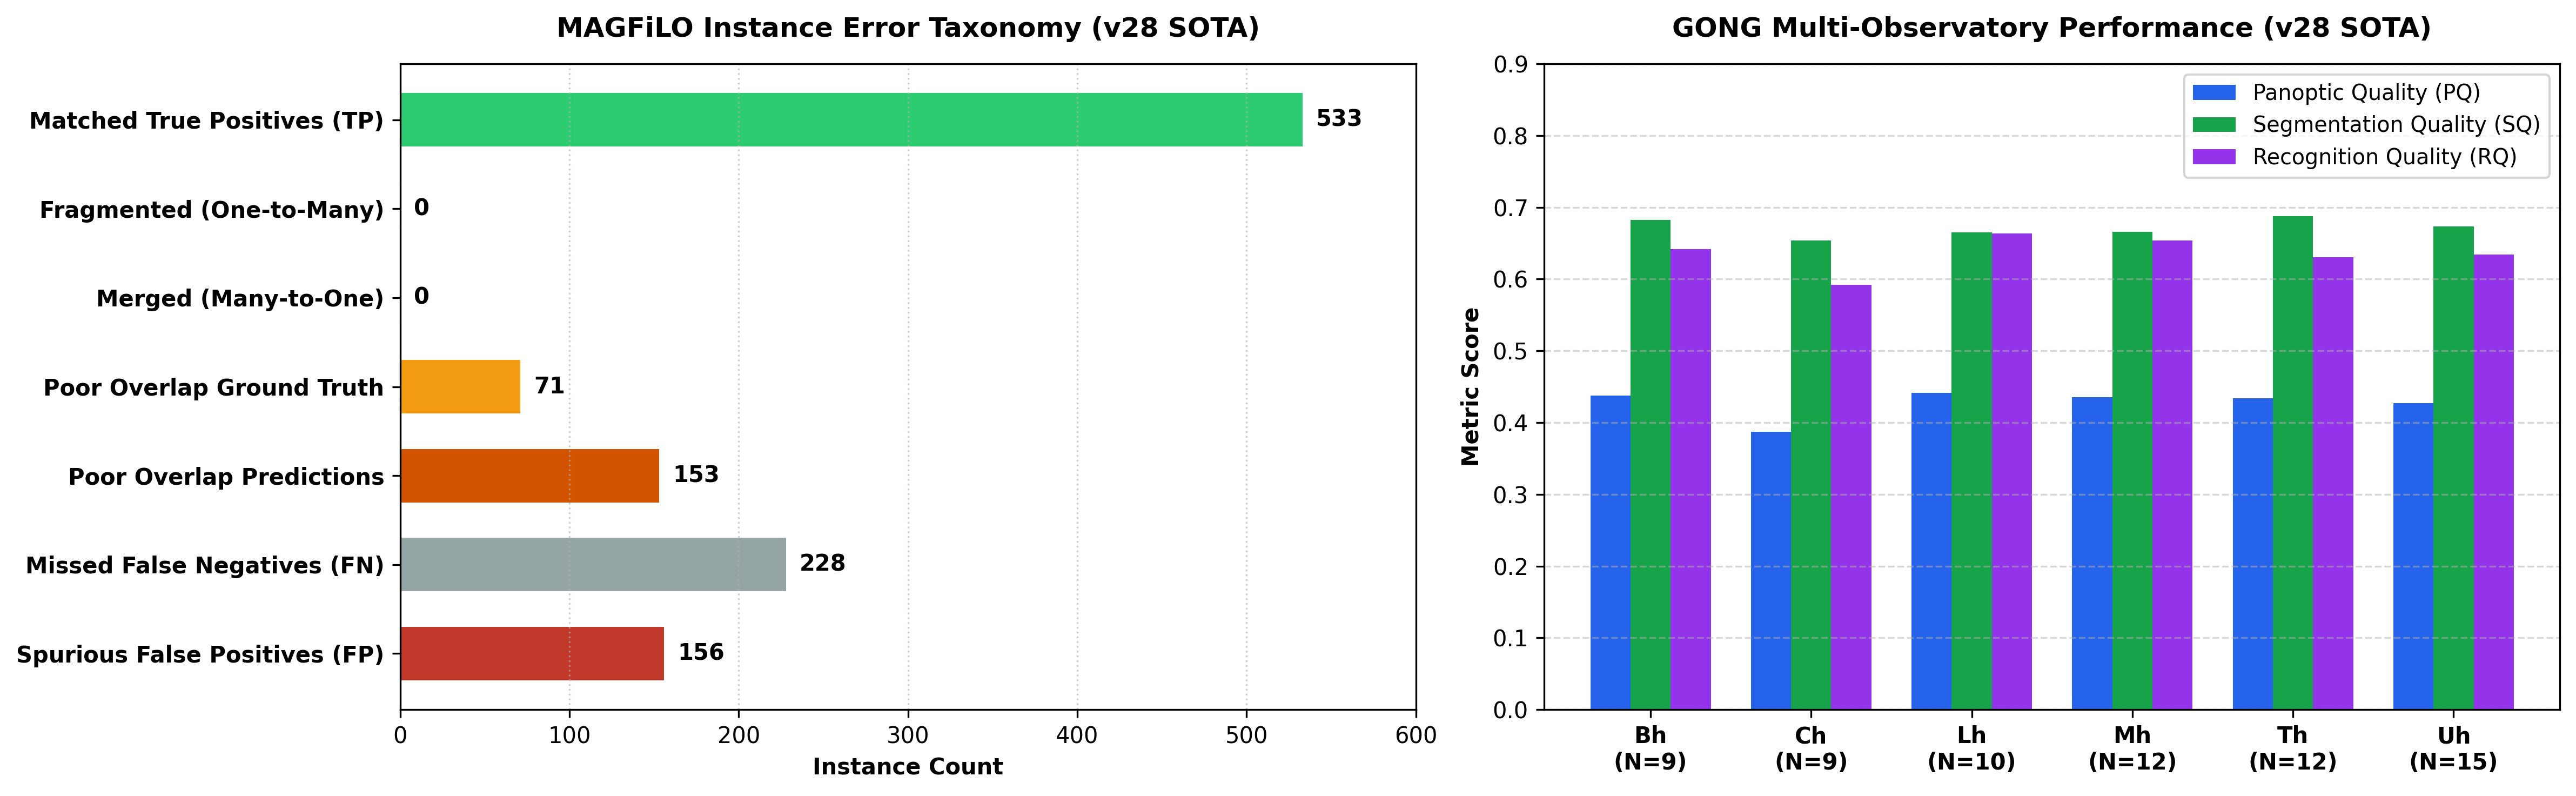
\includegraphics[width=\linewidth]{figures/taxonomy_observatory_analysis.png}
    \caption{Error taxonomy distribution (left) and per-observatory metric comparison (right), showing dominant True Positive matching and balanced cross-station performance.}
    \label{fig:taxonomy_obs}
\end{figure}

\subsection{Strengths, Weaknesses, and Future Directions}
\textbf{Strengths:}
\begin{itemize}
    \item \textbf{Metric Alignment:} Our loss formulation and directional post-processing directly optimize the non-linear $\text{IoU} > 0.50$ matching mechanics.
    \item \textbf{Physics-Based Generalization:} Directional dilation along the Polarity Inversion Line respects the astrophysical magnetic geometry, preventing lateral over-merging.
    \item \textbf{High Efficiency:} Zero-compute ingestion of pre-converged checkpoints allows full validation and test generation in $< 35\text{ minutes}$ on a single GPU.
\end{itemize}

\textbf{Weaknesses \& Limitations:}
\begin{itemize}
    \item \textbf{Two-Stage Instance Extraction:} Converting semantic probabilities to instances via morphological connected components remains an approximation of true end-to-end instance segmentation.
    \item \textbf{Active Region Granulation Clusters:} Highly disturbed active regions occasionally trigger false positives that survive morphological filtering.
\end{itemize}

\textbf{Future Directions:}
We plan to investigate: (1) State-Space Models (Vision Mamba / VMamba) enabling native $2048 \times 2048$ full-disk attention with linear complexity; (2) multi-modal physics fusion combining H-$\alpha$ with SDO/HMI line-of-sight magnetograms ($B_{\text{LOS}}$) to guide flux rope connectivity directly by magnetic polarity; and (3) query-based Panoptic Transformers (Mask2Former) for end-to-end instance delineation.

% ==================================== %
%            ACKNOWLEDGMENT            %
% ==================================== %
\section{Acknowledgment}\label{sec:acknowledgment}
    The organization of the Filament Segmentation Challenge 2026 is partially supported by the U.S. National Science Foundation (NSF) under Grant No. 2209912 and 2433781, directorate for Computer and Information Science and Engineering (CSE), and Office of Advanced Cyberinfrastructure (OAC), and Grant No. 2511630, AST Division Of Astronomical Sciences and MPS Directorate for Mathematical and Physical Sciences.

    The Filament Segmentation Challenge 2026 is sponsored by the U.S. National Science Foundation (NSF) National Solar Observatory (NSO). 

    This work utilizes GONG data obtained by the NSO Integrated Synoptic Program, managed by the National Solar Observatory, which is operated by the Association of Universities for Research in Astronomy (AURA), Inc. under a cooperative agreement with the National Science Foundation and with contribution from the National Oceanic and Atmospheric Administration. The GONG network of instruments is hosted by the Big Bear Solar Observatory, High Altitude Observatory, Learmonth Solar Observatory, Udaipur Solar Observatory, Instituto de Astrofísica de Canarias, and Cerro Tololo Interamerican Observatory.

\bibliographystyle{ACM-Reference-Format}
\bibliography{main}

\end{document}
